\documentclass{beamer}
%
% Choose how your presentation looks.
%
% For more themes, color themes and font themes, see:
% http://deic.uab.es/~iblanes/beamer_gallery/index_by_theme.html
%
\mode<presentation>
{
  \usetheme{default}      % or try Darmstadt, Madrid, Warsaw, ...
  \usecolortheme{beaver} % or try albatross, beaver, crane, ...
  \usefonttheme{default}  % or try serif, structurebold, ...
  \setbeamertemplate{navigation symbols}{}
  \setbeamertemplate{caption}[numbered]
} 

\usepackage[english]{babel}
\usepackage[utf8x]{inputenc}
\usepackage{hyperref}
\hypersetup{
    colorlinks=true,
    linkcolor=blue,
    filecolor=magenta,      
    urlcolor=blue,
}

\title[Communication Protocols]{Communication Protocols}
\author{Andrés Pérez}
\institute{Digital Lutherie\\Master en Música para Experiencias del Entretenimiento\\ENTI-UB}
\date{2018/2019}
\newcommand\blfootnote[1]{%
  \begingroup
  \renewcommand\thefootnote{}\footnote{#1}%
  \addtocounter{footnote}{-1}%
  \endgroup
}

\AtBeginSection[]
{
\begin{frame}{Outline}
    \tableofcontents[currentsection] 
\end{frame}
}

\begin{document}

\begin{frame}
  \titlepage
\end{frame}



\begin{frame}{Outline}
 \tableofcontents
\end{frame}

%%%%%%%%%%%%%%%%%%%%%%%%%%%%%%%%%%%%%%%%%%%%%%%%%%
%%%%%%%%%%%%%%%%%%%%%%%%%%%%%%%%%%%%%%%%%%%%%%%%%%
%%%%%%%%%%%%%%%%%%%%%%%%%%%%%%%%%%%%%%%%%%%%%%%%%%
\section{MIDI}

%%%%%%%%%%%%%%%%%%%%%%%%%%%%%%%%%%%%%%%%%%%%%%%%%%
\subsection{Description}

\begin{frame}{MIDI - Description}
    \begin{figure}[h]
        
\includegraphics[width=\textwidth]{440px-MIDI_LOGO.jpg}
    \end{figure}
\end{frame}

\begin{frame}{MIDI - Description}
\textit{"MIDI (short for \textit{Musical Instrument Digital Interface}) is a technical standard that describes a communications protocol, digital interface, and electrical connectors that connect a wide variety of electronic musical instruments, computers, and related audio devices\footnote{https://en.wikipedia.org/wiki/MIDI}."}
\end{frame}

\begin{frame}{MIDI - Description}
   \textit{"MIDI (short for \textit{Musical Instrument Digital Interface}) is a technical standard that describes a \textbf{communications protocol},\textbf{ digital interface}, and \textbf{electrical connectors} that connect a wide variety of electronic musical instruments, computers, and related audio devices\footnote{https://en.wikipedia.org/wiki/MIDI}."}
\end{frame}

%%%%%%%%%%%%%%%%%%%%%%%%%%%%%%%%%%%%%%%%%%%%%%%%%%
\subsection{History}

\begin{frame}{MIDI - History}
   Before MIDI...
   \vspace{5mm}
   \begin{itemize}
       \item General incompatibility of audio hardware.
       \item Some "standards"...
       \begin{itemize}
           \item CV/Gate: analog consequence of modular synths.
           \item DCB (Digital Control Bus): Protocol by Roland.
       \end{itemize}
   \end{itemize}
\end{frame}

\begin{frame}{MIDI - History}
    \begin{figure}[h]
        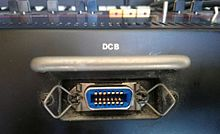
\includegraphics[width=\textwidth]{220px-DCB_interface.jpg}
    \end{figure}
\end{frame}

\begin{frame}{MIDI - History}
    \begin{itemize}
        \item Itakuro Kakehashi (founder of Roland) started conversations with audio hardware companies in 1981.
        \item AES standard proposal discussion: Roland, Yamaha, Korg, Kawai and Sequencial Circuits. 
        \item Official announcement by Moog in 1982 in the \textit{Keyboard} magazine.
        \item First synths implementing MIDI: Roland Jupiter-6 and Sequencial Circuit Prophet 600 (1982)
        \item MIDI 1.0 specification published in 1983.
    \end{itemize}
\end{frame}

\begin{frame}{MIDI - History}
    "The creative possibilities brought about by MIDI technology are credited for helping revive the music industry in the 1980s"\footnote{Shuker, Roy. Understanding Popular Music. London: Routledge, 1994. p.286}.\\
    \vspace{5mm}
    "MIDI revolutionized the music industry, and its continued use is a good measure of the success of the standard"\footnote{Phillips, Dave. An Introduction to OSC. Linux Journal. https://www.linuxjournal.com/content/introduction-osc}.
\end{frame}

%%%%%%%%%%%%%%%%%%%%%%%%%%%%%%%%%%%%%%%%%%%%%%%%%%
\subsection{Specifications}

\begin{frame}{MIDI - Specifications}
    MIDI 1.0: Two specification levels:
    \begin{itemize}
        \item Hardware Transport
        \item Message Format
    \end{itemize}
\end{frame}

\begin{frame}{MIDI - Specifications}
    Hardware Transport\\
    \vspace{5mm}
    \begin{itemize}
        \item Simplex (one way data transmission)
        \item Asynchronous serial
        \item Rate: 3.125 kBps
        \item 5-pin DIN connector
    \end{itemize}
\end{frame}

\begin{frame}{MIDI - Specifications}
    \begin{figure}[h]
        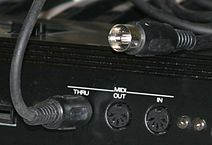
\includegraphics[width=\textwidth]{212px-Midi_ports_and_cable.jpg}
    \end{figure}
\end{frame}

\begin{frame}{MIDI - Specifications}
    Message Format\footnote{For more info check https://www.midi.org/specifications-old/item/table-1-summary-of-midi-message}\\
    \vspace{5mm}
    Different message types:
    \begin{itemize}
        \item Channel Voice
        \item Channel Mode
        \item System
    \end{itemize}
    
    
\end{frame}

\begin{frame}{MIDI - Specifications}
    Channel Voice Messages\\
    \begin{itemize}
        \item 7 bit value range (128 different values)
        \item 4 bit channel range (16 different channels)
    \end{itemize}
    \vspace{5mm}
    \begin{itemize}
        \item Note On / Note Off
        \item Control Change (CC)
        \item Program Change
        \item Pitch Bend Change
        \item Aftertouch
    \end{itemize}
\end{frame}

\begin{frame}{MIDI - Specifications}
    Channel Voice Messages\\
    \vspace{5mm}
    \textbf{Note On / Note Off}\\
    $[$Channel Note Velocity$]$
    \vspace{5mm}
    \begin{itemize}
        \item Start/end of single musical event
        \item Note range: $C_{-1}$ to $G_9$, 8.176 to 12.544 Hz\footnote{Grand piano ranges 88 notes from $A_0$ to $C_8$.}.
        \item Two implementations of note end:
        \begin{itemize}
            \item \textit{Note Off} message in a note previously activated by \textit{Note On}
            \item \textit{Note On} message with 0 velocity
        \end{itemize}
    \end{itemize}
\end{frame}

\begin{frame}{MIDI - Specifications}
    Channel Voice Messages\\
    \vspace{5mm}
    \textbf{Control Change}\\
    $[$Channel ControlNumber Value$]$
    \vspace{5mm}
    \begin{itemize}
        \item Sends information about the value of a control
        \item Commonly used for sliders, knobs...
        \item Last 8 control number values are reserved (\textit{Channel Mode Messages})
    \end{itemize}
\end{frame}

\begin{frame}{MIDI - Specifications}
    Channel Voice Messages\\
    \vspace{5mm}
    \textbf{Pitch Bend}\\
    $[$Channel Value$]$
    \vspace{5mm}
    \begin{itemize}
        \item Changes \textbf{global} pitch in +-2 semitones
        \item Special resolution: 16384 values
    \end{itemize}
\end{frame}

\begin{frame}{MIDI - Specifications}
    Channel Voice Messages\\
    \vspace{5mm}
    \textbf{Aftertouch (Note)}\\
    $[$Channel Note Value$]$
    \vspace{5mm}
    \begin{itemize}
        \item Allows note expressivity (tremolo, vibrato)
        \item Not always implemented...
    \end{itemize}
\end{frame}

\begin{frame}{MIDI - Specifications}
    Channel Mode Messages\\
    \vspace{5mm}
    \begin{itemize}
        \item 8 last control numbers of the CC message
        \item Special sound messages:
        \begin{itemize}
            \item \textit{All Sound Off}
            \item \textit{Reset All Controllers}
            \item \textit{Local Control}
            \item \textit{All Notes Off}
            \item \textit{Omni/Poly modes}
        \end{itemize}
    \end{itemize}
\end{frame}

\begin{frame}{MIDI - Specifications}
    System Messages\\
    \vspace{5mm}
    Some non-musical message definitions:
    \begin{itemize}
        \item Manufacturer exclusive messages (\textit{SysEx})
        \item Playback transport
        \item Time Codes
        \item ...
    \end{itemize}
\end{frame}

\begin{frame}{MIDI - Specifications}
    Some drawbacks...\\
    \begin{itemize}
        \item Slow transmission rate
        \item Non-flexible music representation (biased towards 12 tone equal-temperament, western timing representation...)
        \item Designed for keyboards
        \item Insufficient numeric resolution in CC
        \item ...
    \end{itemize}
    ... but still a successful technology (almost) 40 years after!
\end{frame}


%%%%%%%%%%%%%%%%%%%%%%%%%%%%%%%%%%%%%%%%%%%%%%%%%%
\subsection{Extensions}

\begin{frame}{MIDI - Extensions}
    USB-MIDI\footnote{For more info check https://www.midi.org/articles-old/basic-of-usb}\\
    \vspace{5mm}
    \begin{itemize}
        \item 5-pin DIN is nowadays not very popular...\\
        \item Implementation of MIDI as Audio Class-Compilant Profile
        \item USB is much faster: one connection might support up to 16 independent MIDI streams 
    \end{itemize}
\end{frame}

\begin{frame}{MIDI - Extensions}
    General MIDI\\
    \vspace{5mm}
    \centering{\textbf{General MIDI is \_NOT\_ MIDI}}
\end{frame}

\begin{frame}{MIDI - Extensions}
    General MIDI\\
    \vspace{5mm}
    \begin{itemize}
        \item Sound specification for instruments responding to MIDI messages
        \item Attempt to standardize the sound produced by MIDI instruments/synths
    \end{itemize}
\end{frame}

\begin{frame}{MIDI - Extensions}
    General MIDI\\
    \vspace{5mm}
    Required features:
    \begin{itemize}
        \item 24 simultaneous voices
        \item Note velocity
        \item Usage of all 16 channels (channel 10 reserved for percussion)
        \item Polyphony
    \end{itemize}
\end{frame}

\begin{frame}{MIDI - Extensions}
    General MIDI\\
    \vspace{5mm}
    Required features:
    \begin{itemize}
        \item 24 simultaneous voices
        \item Note velocity
        \item Usage of all 16 channels (channel 10 reserved for percussion)
        \item Polyphony
    \end{itemize}
\end{frame}

\begin{frame}{MIDI - Extensions}
    \begin{figure}[h]
        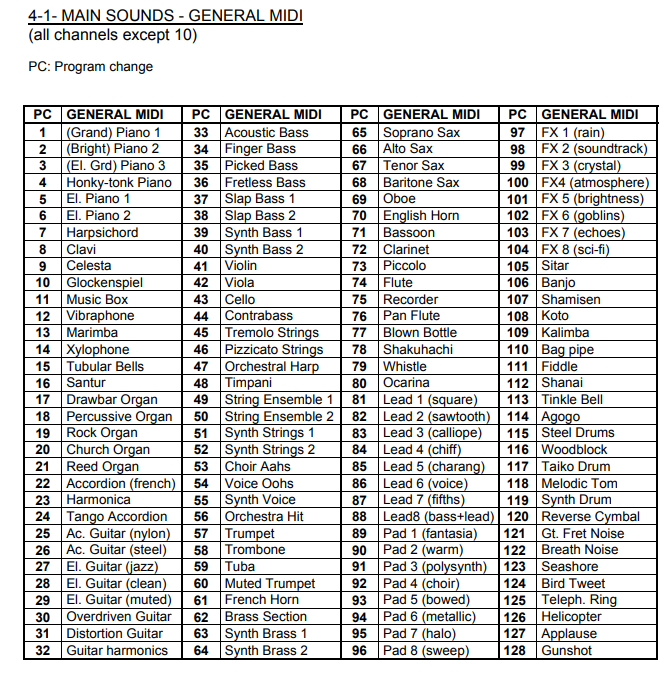
\includegraphics[width=0.7\textwidth]{generalmidi.png}
    \end{figure}
\end{frame}

\begin{frame}{MIDI - Extensions}
    \begin{figure}[h]
        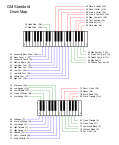
\includegraphics[width=0.5\textwidth]{119px-GM_Standard_Drum_Map_on_the_keyboard.png}
    \end{figure}
    \blfootnote{By Manudiclemente - text editor, CC BY-SA 3.0, https://commons.wikimedia.org/w/index.php?curid=19937484}
\end{frame}

\begin{frame}{MIDI - Extensions}
    MIDI 2.0\footnote{For more info check https://www.midi.org/articles-old/the-midi-manufacturers-association-mma-and-the-association-of-music-electronics-industry-amei-announce-midi-2-0tm-prototyping}\\
    \vspace{5mm}
    \begin{itemize}
        \item Extends limitations of MIDI 1.0
        \item Backwards-compatible
        \item Announced in January 2019
        \item Industry standard: Ableton/Cycling '74, Art+Logic, Bome Software, Google, imitone, Native Instruments, Roland, ROLI, Steinberg, TouchKeys, and Yamaha
    \end{itemize}
\end{frame}

\begin{frame}{MIDI - Extensions}
    \begin{figure}[h]
        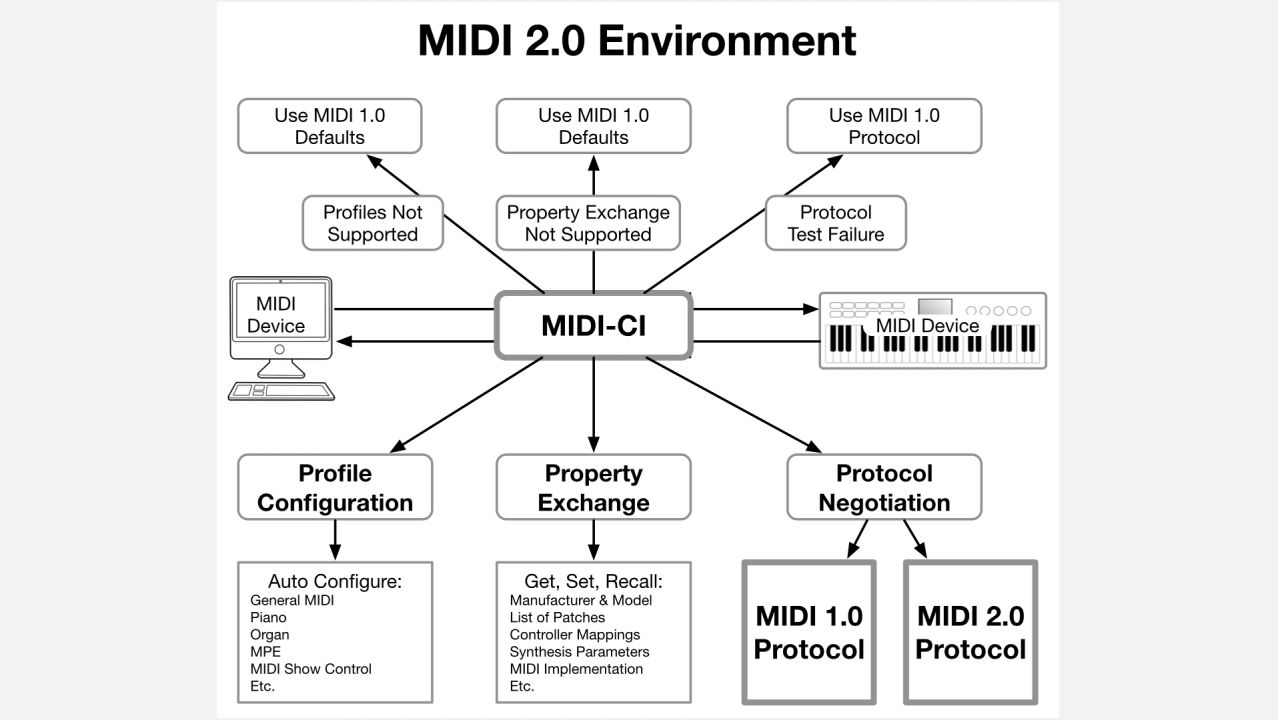
\includegraphics[width=1.2\textwidth]{MIDI-20.jpg}
    \end{figure}
\end{frame}



%%%%%%%%%%%%%%%%%%%%%%%%%%%%%%%%%%%%%%%%%%%%%%%%%%
%%%%%%%%%%%%%%%%%%%%%%%%%%%%%%%%%%%%%%%%%%%%%%%%%%
%%%%%%%%%%%%%%%%%%%%%%%%%%%%%%%%%%%%%%%%%%%%%%%%%%
\section{OSC}

%%%%%%%%%%%%%%%%%%%%%%%%%%%%%%%%%%%%%%%%%%%%%%%%%%
\subsection{Description}

\begin{frame}{OSC - Description}
    \textit{Open Sound Control} (OSC) is a protocol for communication among computers, sound synthesizers, and other multimedia devices that is optimized for modern networking technology. Bringing the benefits of modern networking technology to the world of electronic musical instruments, OSC's advantages include interoperability, accuracy, flexibility, and enhanced organization and documentation\footnote{http://opensoundcontrol.org/introduction-osc}.
\end{frame}

\begin{frame}{OSC - Description}
    Features\footnote{http://opensoundcontrol.org/introduction-osc}:
    \begin{itemize}
        \item Open-ended, dynamic, URL-style symbolic naming scheme
        \item Symbolic and high-resolution numeric argument data
        \item Pattern matching language to specify multiple recipients of a single message
        \item High resolution time tags
        \item "Bundles" of messages whose effects must occur simultaneously
        \item Query system to dynamically find out the capabilities of an OSC server and get documentation
  \end{itemize}  
\end{frame}

%%%%%%%%%%%%%%%%%%%%%%%%%%%%%%%%%%%%%%%%%%%%%%%%%%
\subsection{Specifications}

\begin{frame}{OSC - Specifications}
    Atomic data types:
    \begin{itemize}
        \item int32: 32 bit fixed-point
        \item OSC-timetag: 64 bit fixed-point
        \item float32: 32 bit IEEE 754 floating-point
        \item OSC-string: ASCII character
        \item OSC-blob: arbitrary binary data
  \end{itemize}  
\end{frame}

\begin{frame}{OSC - Specifications}
    OSC Message:
    \begin{itemize}
        \item OSC Address: string starting with '/'
        \item OSC Type Tag: character representing the data type sent
        \item OSC Argument: actual values sent, interpreted by the type tags
    \end{itemize}  
    \vspace{5mm}
    OSC Bundle
    \begin{itemize}
        \item OSC Time Tag
        \item OSC Bundle Element: any OSC Message or OSC Bundle
    \end{itemize}  
\end{frame}

\begin{frame}{OSC - Specifications}
    OSC Message examples:\\
    \vspace{5mm}
    \begin{itemize}
        \item /this/is/an/OSC/message
        \item /synth/1/gain, 0.5
        \item /foo/bar, 1, 'asdf', 3.141592
    \end{itemize}  
\end{frame}

\begin{frame}{OSC - Specifications}
    So... where is the sound?
    \begin{itemize}
        \item OSC is in fact not a protocol in the same sense as MIDI, but rather a \textit{content format}.
        \item That means that \textbf{there is not} a standard way of expressing sound/music information\footnote{Despite there have been some attempts... https://github.com/fabb/SynOSCopy/wiki}.
        \item OSC just unifies how to send data between applications, but not how this data looks like...
    \end{itemize}
\end{frame}

\begin{frame}{OSC - Specifications}
    \begin{itemize}
        \item OSC is a popular data sharing protocol in multimedia applications.
        \begin{itemize}
            \item DAWS: Logic, Reaper, Ardour, Traktor...
            \item Sound programming languages: Max/MSP, Pure Data, SuperCollider, Sonic Pi...
            \item Graphics: Blender, OpenFrameworks, UnrealEngine, Processing...
            \item Hardware Controllers: Monome, Lemur...
        \end{itemize}
        \item OSC and MIDI are not direct competitors!\footnote{Interesting reading: https://www.midi.org/articles-old/white-paper-comparison-of-midi-and-osc}
    \end{itemize}
\end{frame}

\end{document}
